
\documentclass[tikz,border=7pt]{standalone}

\usepackage{amsmath,amssymb}
\usepackage{tikz}
\usepackage{verbatim}
\usetikzlibrary{arrows.meta,positioning,calc}

\definecolor{inputblue}{RGB}{220,220,247}
\definecolor{outputblue}{RGB}{215,215,246}
\definecolor{biaspink}{RGB}{248,220,222}
\definecolor{activationgreen}{RGB}{216,245,216}

\begin{document}

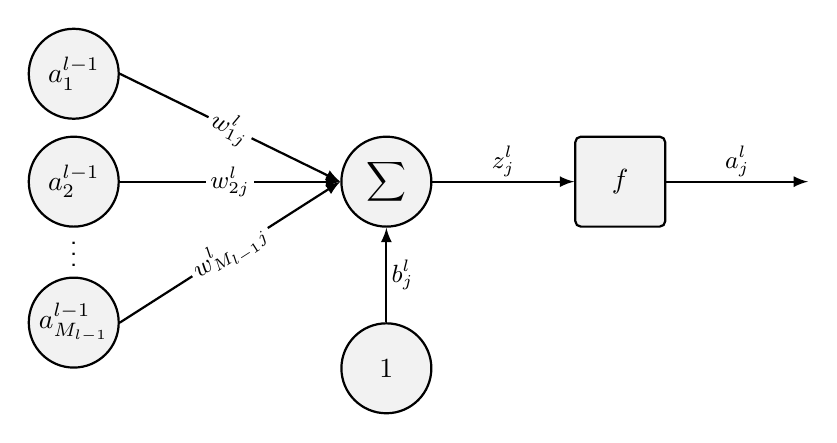
\begin{tikzpicture}[
    >=Latex,
    font=\sffamily,
    node distance=1.5cm,
    line/.style={
        -latex,
        thick
    },
    neuron/.style={
        circle,
        minimum size=3.25em,
        inner sep=0pt,
        draw,
        fill=gray!10,
        thick
    },
    input/.style={neuron},
    target/.style={neuron},
    bias/.style={neuron},
    operator/.style={neuron},
    activation/.style={
        rectangle,
        rounded corners=2pt,
        minimum size=3.25em,
        inner sep=0pt,
        draw,
        fill=gray!10,
        thick
    },
    loss/.style={
        draw=black!60,
        dashed,
        line width=0.65pt,
        minimum width=28mm,
        minimum height=13mm,
        inner sep=5pt
    },
    annotation/.style={
        text=black!65,
        font=\small
    },
    weight/.style={
        fill=white,
        inner sep=1.5pt,
        font=\small
    }
]

% Input features
\node[input] (x1) {$a_1^{l-1}$};
\node[input, below=2mm of x1] (x2) {$a_2^{l-1}$};
\node[below=-1.5mm of x2] (dots) {$\vdots$};
\node[input, below=0mm of dots] (xp) {$a_{M_{l-1}}^{l-1}$};

% Linear combination
\node[operator, right=28mm of x2] (sum)
    {$\displaystyle\sum$};

% Bias
\node[bias, below=12mm of sum] (one) {$1$};

% Activation
\node[activation, right=18mm of sum] (sigma)
    {$f$};

% Input connections
\foreach \x/\n in {x1/1,x2/2} {
    \draw[line] (\x.east) -- (sum.west)
        node[weight, midway, sloped] {$w_{\n j}^l$};
}
\draw[line] (xp.east) -- (sum.west)
    node[weight, midway, sloped] {$w_{M_{l-1}j}^l$};

% Bias connection
\draw[line] (one.north) -- (sum.south)
    node[weight, midway, right] {$b_j^l$};

% Forward pass
\draw[line] (sum.east) -- (sigma.west)
    node[weight, midway, above] {$z_j^l$};

% Output
\draw[line] (sigma.east) -- ++(18mm,0)
    node[weight, midway, above] {$a_j^l$};

% Linear predictor equation
\begin{comment}
\node[above=14mm of sum, anchor=center]
    (equation)
    {$\displaystyle z_j^l = \sum_{i=1}^{M_{l-1}} w_{ij}^l a_i^{l-1}+b_j^l$};
\end{comment}

\end{tikzpicture}

\end{document}
